\section{Results and Discussion} \label{ch:lfs:results}

The experimental evaluation of the various methods that we developed is done in three
phases. First, we investigated how well the proposed models can explain the users' ratings over sets in the dataset we obtained from a subset of Movielens users
(described in Section~\ref{ch:lfs:dataset}). Second, we evaluated the performance of the methods using the synthetically
generated datasets in order to assess how well the underlying optimization algorithms
can recover the underlying data generation models and achieve good prediction
performance at either the set- or item-level. Note that unless otherwise specified,  we report the average of RMSEs of all the
synthetic datasets as the final RMSE values for each rank and proposed approach. Finally, we evaluated the prediction performance achieved by the proposed methods at both the set- or item-level in the real dataset.


%==========================================================================
\subsection{Fit of different rating models} \label{ch:lfs:fit_rating_model}
In order to determine how well the proposed models can explain the ratings that the
users in our dataset provided, we performed the following analysis. We selected
sets with standard deviation of at least 0.5, and included only those users who
have rated at least 20 such sets. This left us with 17,552 sets rated by 493
users.

To study the \ES model, for each set rated
by a user we created all the possible subsets having either $k$ lowest or $k$
highest rated items for all the possible values of $k$ $\in$ [1, 5], i.e., nine
extremal subsets.
We computed the error between the average rating of items in the extremal
subsets and the rating provided by a user on a set. Similarly, we computed the
error over the remaining sets for a user and selected that subset among the nine
extremal subsets corresponding to which the user has lowest Root Mean Square
Error (RMSE) for all the sets.
Figure~\ref{fig:extremal} shows the number of users and their corresponding
extremal subset that obtained lowest RMSE for their sets. As can be seen in the
figure, there are certain users for whom the
lowest RMSE on sets corresponds to either $k$ lowest or $k$ highest rated items in a set,
where $k < 5$. This indicates that while providing a rating to a set of items, the user may get
influenced more by a subset of the items in a set rather than  all the items in
the set.


Further, to investigate \VO model, we computed the user's level of pickiness ($\beta_u$) as 
%
\begin{equation} \label{pickinessEq}
  \begin{split}
    \beta_u &= \frac{1}{n_s}\sum_{s = 1}^{n_s} \frac{r_{u}^s - \mu_s} {\sigma_s},
  \end{split}
\end{equation}
%
where $n_s$ is the number of sets rated by user $u$, $r_{u}^s$ denotes the rating
provided by user $u$ on set $s$, $\mu_s$ is the mean rating of the items in set $s$
and $\sigma_s$ is the standard deviation of the ratings of the items in set $s$.
Figure~\ref{fig:pickiHist} shows the histogram of the  users' level of pickiness. As
can be seen from the figure,  certain users tend to under- or over-rate sets with
high standard deviation, and interestingly more users tend to under-rate sets than
over-rate them. 
%statistical analysis

\begin{figure}[tb]
  \centerline{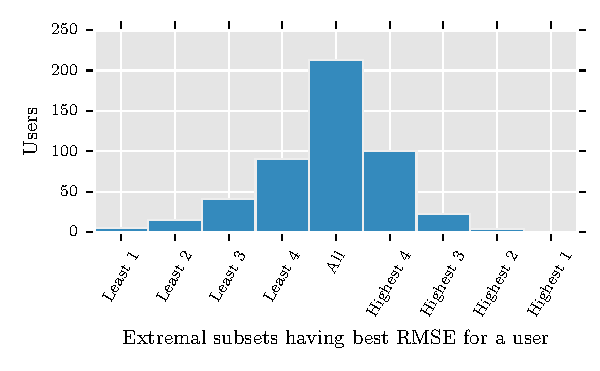
\includegraphics[scale=0.8]{figures/extremalHist.pdf}}
  \caption{The number of users for which their pickiness behavior is explained
  by the corresponding least- and highest-rated subsets of
items.}
  \label{fig:extremal}
\end{figure}


\begin{figure}[tb]
  \centerline{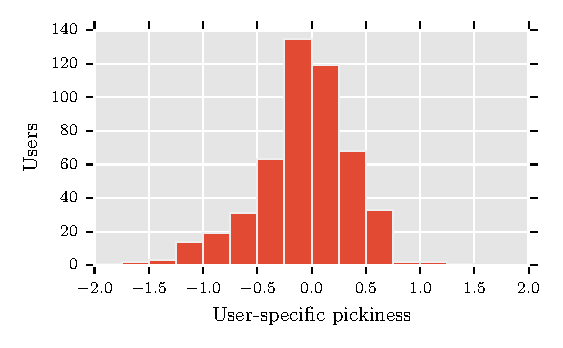
\includegraphics[scale=0.9]{figures/pickiHist.pdf}}
  \caption{The number of users and their computed level of pickiness.}
  \label{fig:pickiHist}
\end{figure}



Additionally, we computed how well the above rating models, i.e., \ES and \VO,
compare against the \ARM model where a user rates
a set as the average of the ratings that he/she gives to the set's items.
We used the user-specific pickiness determined in above analysis for the \ES and
the \VO models to estimate a user's rating on a set.
Table~\ref{table:fit_results} shows the RMSE of the estimated ratings according to different models
and as can be seen in the table both the \ES and the \VO give a better fit to the
real data than \ARM, thereby suggesting that modeling users' level of  pickiness could lead
to better estimates. 



\begin{table}[t]
  \centering
  \caption{Fit of different rating models on the data}
  \label{table:fit_results}
  \begin{threeparttable}
  \def\arraystretch{1.5}
  \begin{tabular}{lccc}
  \hline
      &\multicolumn{1}{c}{\centering \ARM} 
      &\multicolumn{1}{c}{\centering \ES} 
      &\multicolumn{1}{c}{\centering \VO} \\ 
  \hline
  RMSE    & 0.597  & 0.509  & 0.521 \\
  \hline
  \end{tabular}
  \end{threeparttable}
\end{table}




%==========================================================================

\subsection{Performance on the synthetic datasets}


\subsubsection{Accuracy of set- and item-level predictions}
We investigated the performance of the proposed methods for both item- and
set-level predictions on the synthetic datasets.
In addition to the performance of each method on its corresponding dataset,
we also show the performance of the \ARM and \SETAVG methods in Figures~\ref{fig:es_sets_sz}~and~\ref{fig:vo_sets_sz}. 

Figure~\ref{fig:es_sets_sz} shows that \ES outperforms all other methods for 
both set- and item-level predictions for datasets with a large number of sets.
However, for datasets with fewer sets, \ARM  outperforms \ES and
\SETAVG for the set- and item-level predictions. 
Figure~\ref{fig:vo_sets_sz} shows that \VO outperforms all other methods for both
set- and item-level predictions. 
Unlike \ES, \VO performs better than other methods even for the
case when we have fewer sets, and this suggests that \ES needs a
larger number of sets than \VO to recover the underlying characteristics of the
data.

\begin{figure}[t]
  \centerline{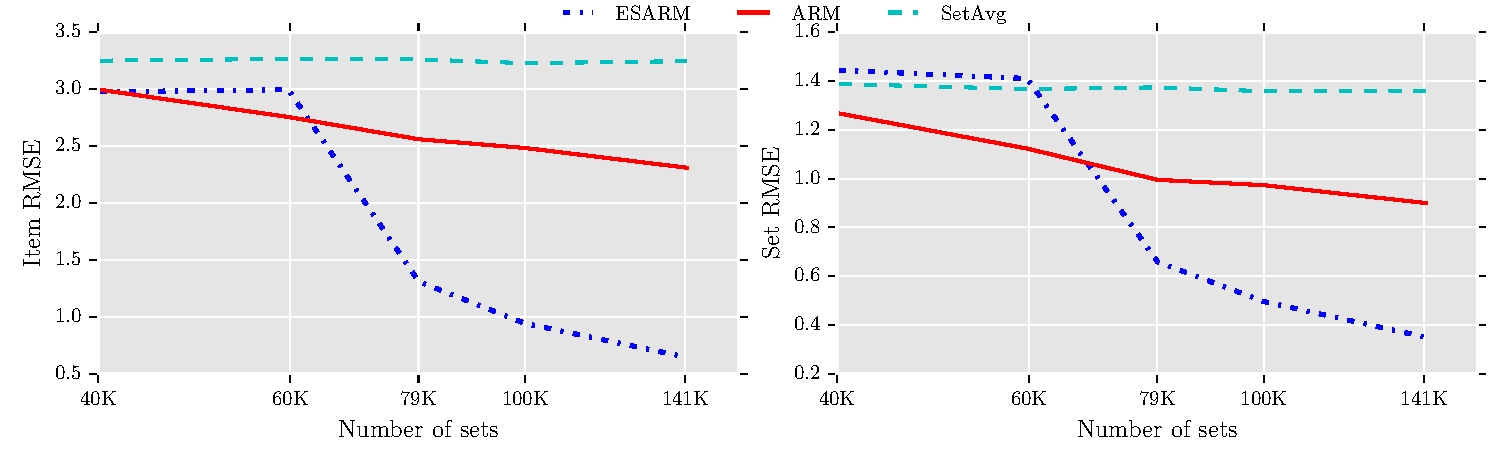
\includegraphics[scale=0.57]{figures/es_sets_sz.pdf}}
  \caption{The average RMSE obtained by the proposed methods on \ES-based datasets with different number of sets.}
  \label{fig:es_sets_sz}
\end{figure}

\begin{figure}[t]
  \centerline{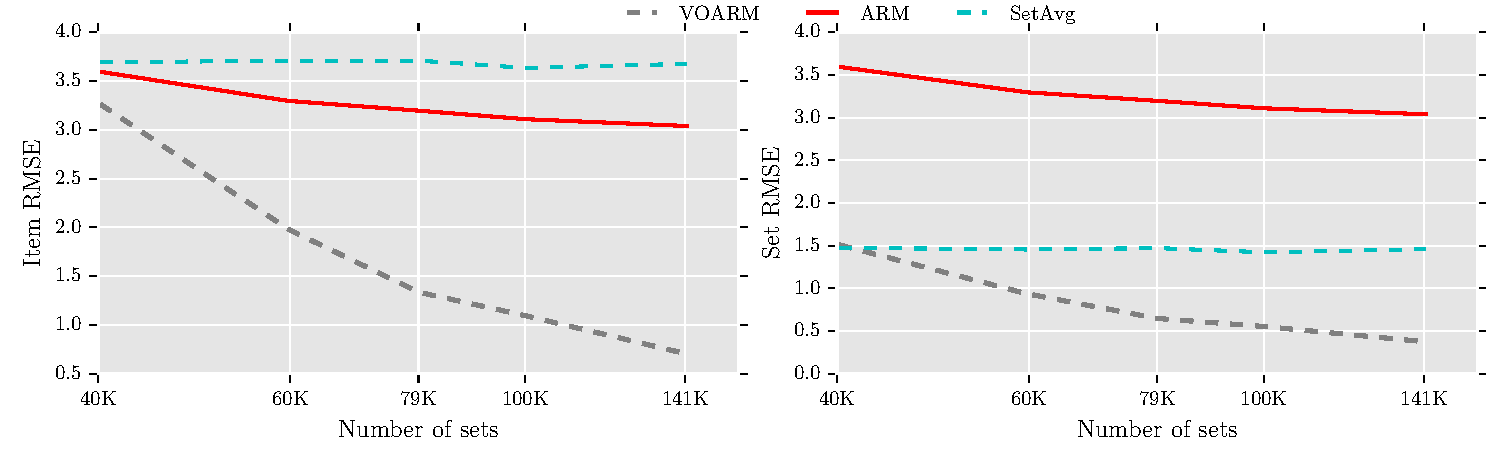
\includegraphics[scale=0.57]{figures/vo_sets_sz.pdf}}
  \caption{The average RMSE obtained by the proposed methods on \VO-based datasets with different number of sets.}
  \label{fig:vo_sets_sz}
\end{figure}




\subsubsection{Recovery of underlying characteristics}\label{ch:lfs:syn_recov}
We examined how well \ES and \VO recover the known underlying characteristics
of the users in the datasets. Figure~\ref{fig:vo_pearson} plots the Pearson correlation coefficient of
the actual and the estimated weights that model the users' level of pickiness in
\VO (i.e., $\beta_u$ parameters). The high values of Pearson correlation
coefficients in the figure
suggests that \VO is able to recover the overall characteristics of the
underlying data. Additionally, this recovery of underlying characteristics
increases with the increase in the number of sets. In order to investigate how well \ES can recover the underlying characteristics,
we computed the fraction of users for whom the extremal subset having the
highest weight ($w_{ui}$) is same as that of the extremal subset used to generate
the rating on sets.   
Figure~\ref{fig:es_sets_recov} shows the percentage of users for whom the extremal subsets are
recovered by \ES. 
As can be seen in the figure, the fraction of users recovered
by \ES increases significantly with the increase in the number of
sets.
The better performance of \ES on the larger
datasets suggests that in order to recover the underlying characteristics of the
data accurately, \ES needs significantly more data than required by
\VO method.

\begin{figure}[t]
 \centerline{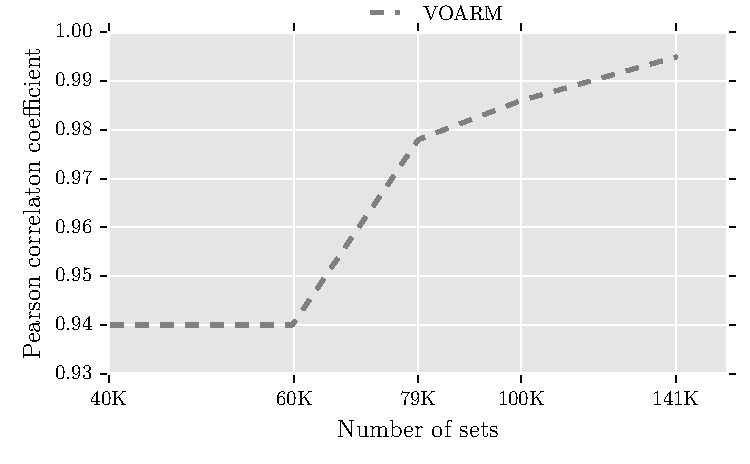
\includegraphics[scale=0.7]{figures/vo_pearson.pdf}}
  \caption{Pearson correlation coefficients of the actual and the estimated
    parameters that model a user's level of pickiness in the \VO model.}
  \label{fig:vo_pearson}
\end{figure}


\begin{figure}[t]
  \centerline{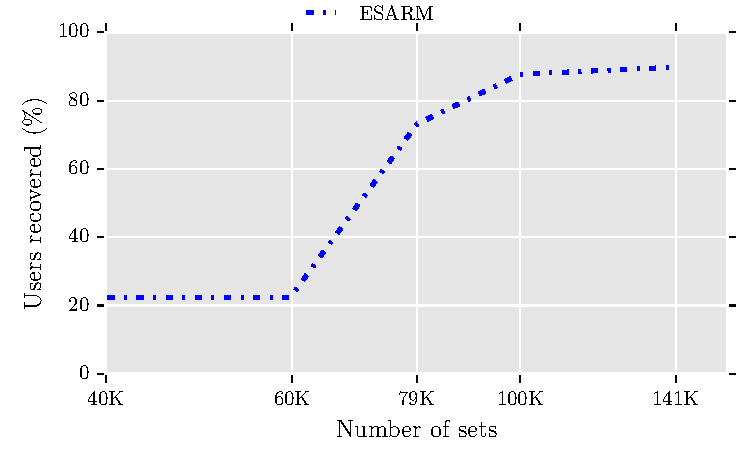
\includegraphics[scale=0.7]{figures/es_sets_recov.pdf}}
  \caption{The percentage of users recovered by \ES, i.e., the users for whom the
    original extremal subset had the highest estimated weight under these models. 
}
  \label{fig:es_sets_recov}
\end{figure}



\iffalse
\begin{figure}[t]
 \centerline{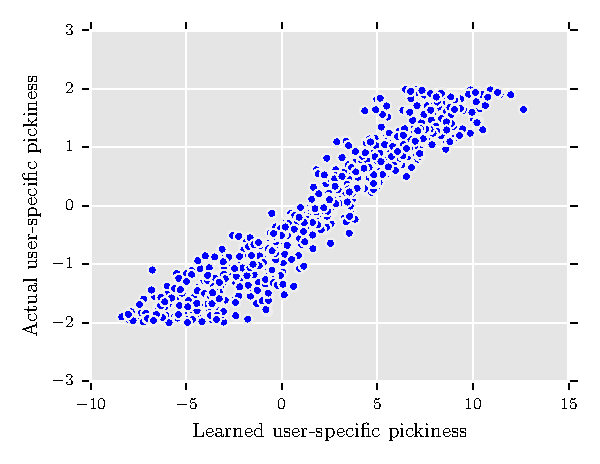
\includegraphics[scale=0.8]{figures/scatter_varmodel_weights.pdf}}
  \caption{A scatter plot of the estimated and actual parameters that model a user's
  level of pickiness in the \VO model.}
  \label{fig:scatter_varmodel_weights}
\end{figure}
\fi



\begin{figure}[t]
  \centerline{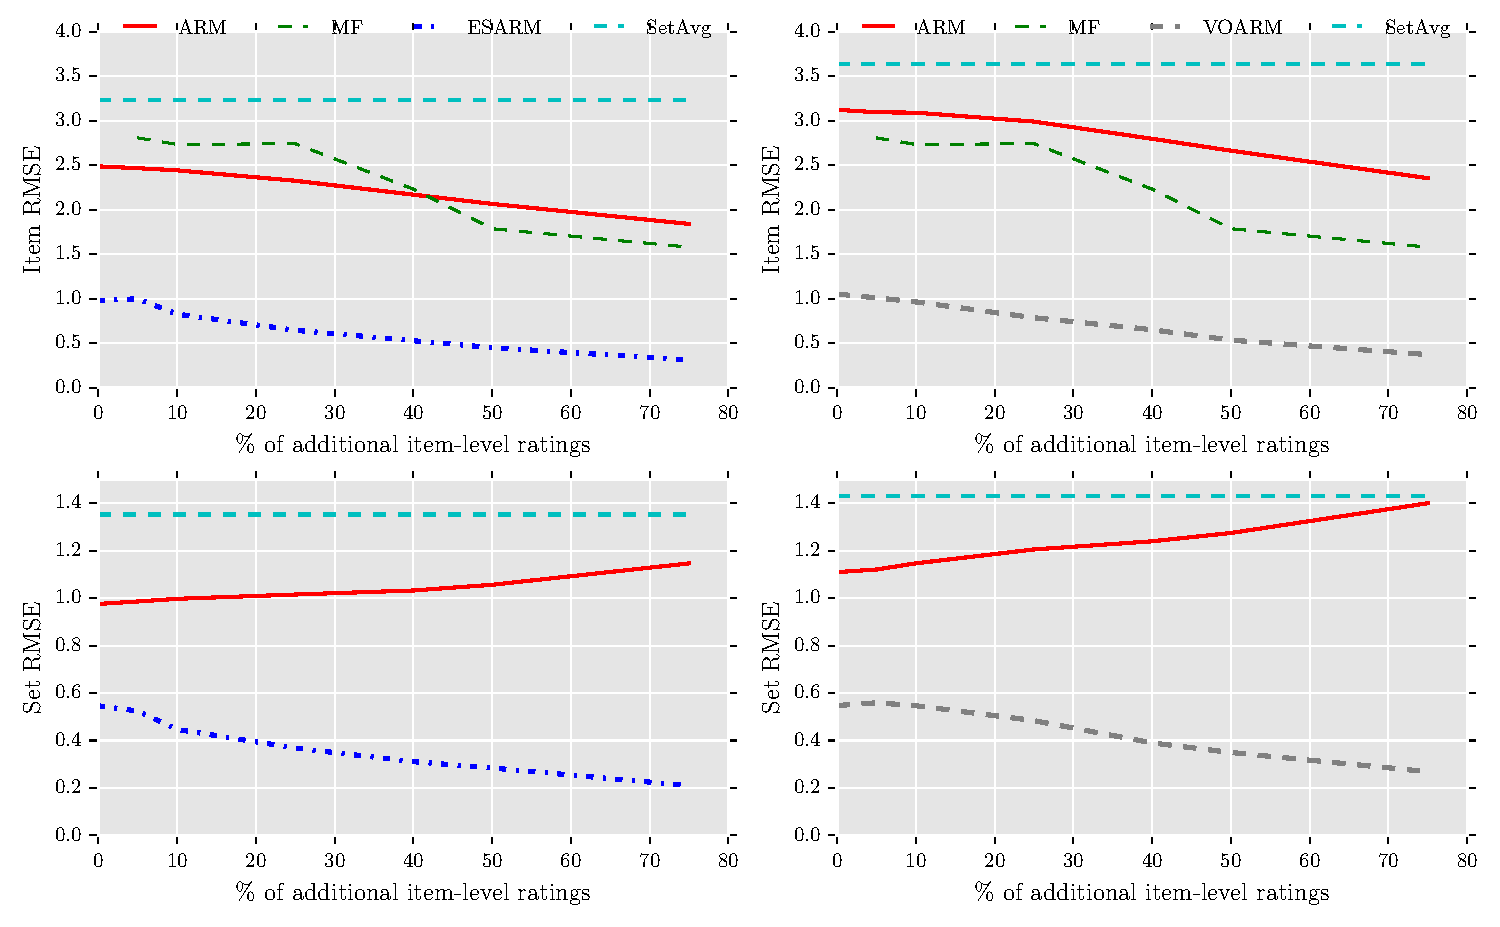
\includegraphics[scale=0.57]{figures/add_items_syn.pdf}}
  \caption{Effect of adding disjoint item-level ratings for the users in \ES-based (left) and \VO-based
  (right) datasets.}
  \label{fig:syn_add_items}
\end{figure}

\begin{figure}[t]
  \centerline{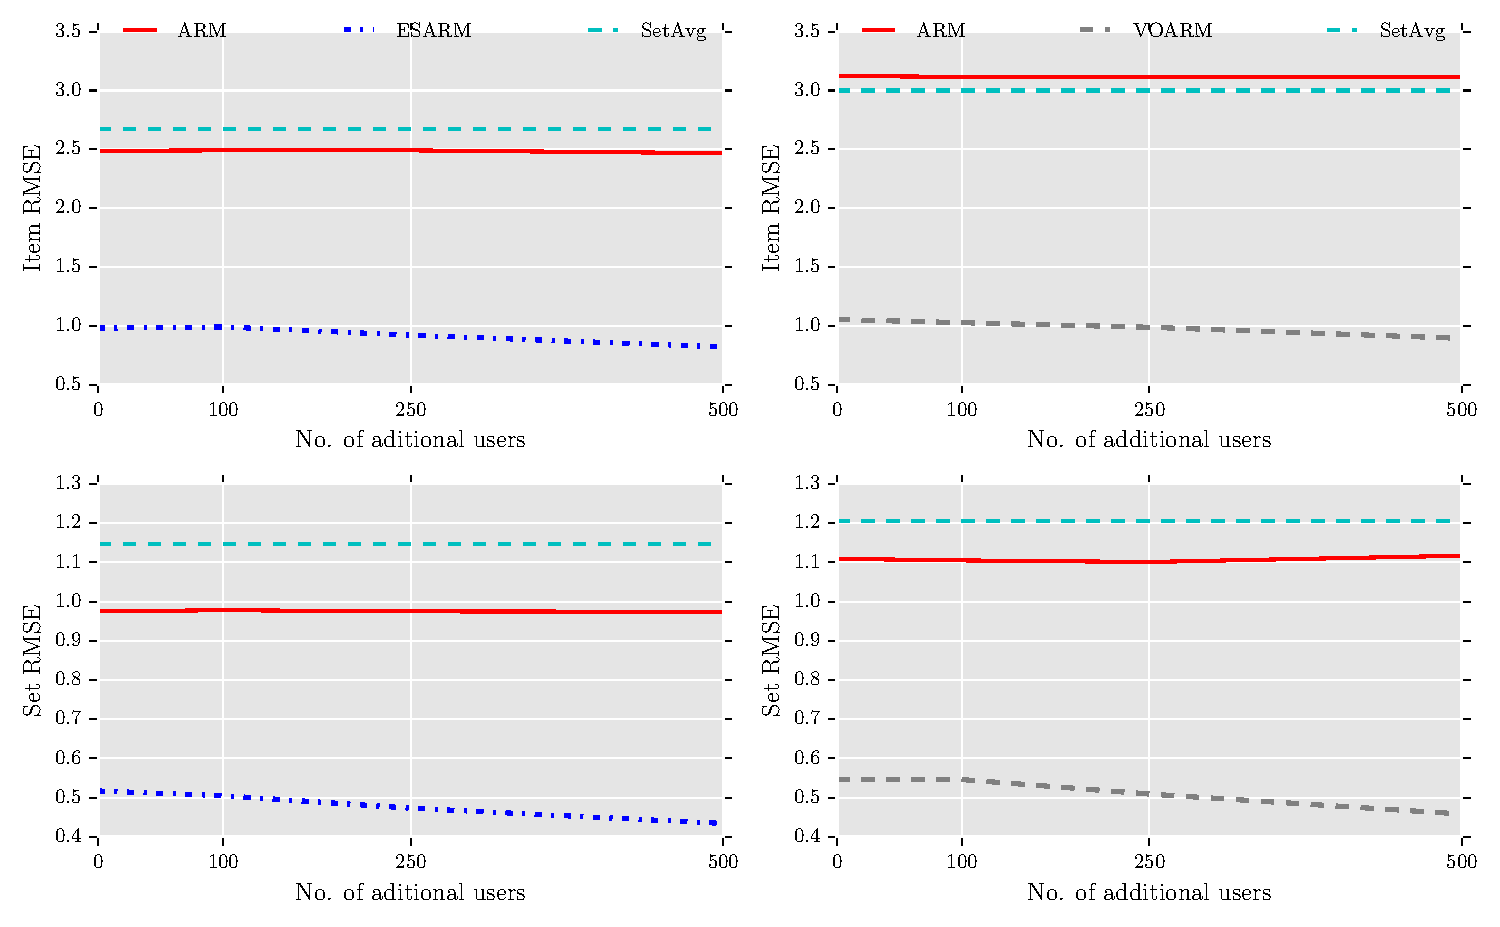
\includegraphics[scale=0.57]{figures/add_users_syn.pdf}}
  \caption{Effect of adding item-level ratings from additional users in \ES-based (left) and \VO-based
  (right) datasets.}
  \label{fig:syn_add_users}
\end{figure}



\subsubsection{Effect of adding item-level ratings}

In most real-world scenarios, in addition to set-level ratings, we will also have
available ratings on individual items as well, e.g., users may provide ratings
on music albums and as well as on tracks in the albums. Also, there may exist
some users that are not concerned about keeping their item-level ratings
private.
To assess how well \ES and \VO  can take advantage of such item-level ratings
we performed three sets of experiments. In the first experiment, we added in the
synthetic datasets a set of item-level ratings for the same set of
users for which we have approximately $100K$ set-level ratings. The number of item-level ratings was
kept to $k$\% of their set-level ratings, where $k \in [5, 75]$, and the items that were added were disjoint
from those that were part of the sets that they rated. Additionally, we used the
matrix factorization (MF) method to estimate the user and item latent
factors by using only the added item-level ratings.
%
In the second experiment, we
selected 100, 250 and 500 additional users (beyond those that exist in the synthetically generated 
datasets) and added a random subset of 50 ratings per user from
the items that belong to the existing users' sets. 
%
In the final experiment, we investigate if using set-level ratings
from one set of users can improve the item-level predictions for another set of
users for whom we have item-level ratings. We selected 500 additional users
($U_b$) and added a random subset of 50  ratings per user from the items that belong to
the sets rated by existing users ($U_a$). 

Figures~\ref{fig:syn_add_items}~and~\ref{fig:syn_add_users} shows the
performance of \ES and \VO on these datasets.
As can be seen from Figure~\ref{fig:syn_add_items}, as we continue to add item-level ratings for the
same set of users who have provided ratings for the sets, there is an increase
in accuracy of both the set- and item-level predictions for  \ES and
\VO. Both \ES and \VO outperform \ARM  with the
availability of more item-level ratings. For the task of item-level rating
prediction, \ES and \VO even outperform MF
which is estimated only based on the additional item-level ratings.
Figure~\ref{fig:syn_add_users} shows how the performance of the proposed methods changes when
item-level ratings are available from another set of users. Similar to the
addition of item-level ratings from the same set of users, \ES and \VO
outperform \ARM with the availability of item-level ratings
from a different set of users.

\begin{table}[bt]
  \centering
  \caption{Average RMSE performance of \ES and \VO for item-level predictions for
  additional users ($U_b$), that have provided only the item-level ratings.}
  \label{table:perf_addu}
  \begin{threeparttable}
  \def\arraystretch{1.5}
    \begin{tabular}{@{\hspace{8pt}}l@{\hspace{8pt}}c@{\hspace{8pt}}c@{\hspace{8pt}}}
      \hline
      & \multicolumn{2}{c}{Item-level RMSE for $U_b$}\\ 
      \cmidrule{2-3}
      Type of ratings & \ES &\VO \\
      \hline
      Item-level ($U_b$) &  2.860 & 2.860\\
      Set-level ($U_a$) + item-level ($U_b$) &  \underline{1.811} & \underline{1.866} \\
      \hline
    \end{tabular}
    \begin{tablenotes}[para,flushleft]
      $U_a$ represents the existing users that have provided ratings at the
      set-level.
      $U_b$ represents the additional 500 users that have provided ratings only at
      item-level and item-level ($U_b$) denotes their item-level ratings. Set-level ($U_a$) refers to the set-level ratings from the
      users in $U_a$.
    \end{tablenotes}
  \end{threeparttable}
\end{table}




Table~\ref{table:perf_addu} shows the performance of item-level predictions for
additional users ($U_b$) after using set-level ratings from existing users
($U_a$).
As can be seen from the table, using set-level ratings
from users in $U_a$ significantly improves the performance of item-level predictions for users
in $U_b$.
That is, using item-level ratings from the additional set of
users and the set-level ratings from the existing users not only
improves the performance for the latter but also for those additional
users who have provided item-level ratings.
The result that the performance of the proposed methods improve with the
addition of item-level ratings suggests that using both item- and
set-level ratings can lead to better item recommendations for the users.


\subsection{Performance on the Movielens-based real dataset}

\begin{table}[t]
  \centering
  \caption{The RMSE performance of the proposed methods with user- and
  item-biases on \MLREALSETS dataset.}
  \label{table:real_wbias_results}
  \begin{threeparttable}
  \def\arraystretch{1.5}
  \begin{tabular}{@{\hspace{10pt}}l@{\hspace{40pt}}c@{\hspace{40pt}}c@{\hspace{10pt}}}
  \hline
    Method & Item & Set\\
  \hline
  SetAvg  & 0.976  & 0.630\\
  \ARM    & \underline{0.971} & 0.624\\
  \ES  & 0.979 & 0.631\\
  \VO     & 0.973 & \underline{0.623}\\ 
  \hline
  \end{tabular}
  \end{threeparttable}
\end{table}

Our final experiment used the proposed approaches (\ARM, \ES, and \VO) to
estimate both set- and item-level rating prediction models using the real
set-level rating dataset that we obtained from \ML users. 

\subsubsection{Accuracy of set- and item- level predictions}
Table~\ref{table:real_wbias_results} shows results for the case when we have
only set-level ratings. 
As can be seen in the table, \ARM outperforms the remaining methods for item-level 
predictions. However, \VO performs somewhat better than \ARM for set-level predictions. The better performance
of \ARM for item-level predictions is not surprising as most of the sets in the dataset
are rated close to the average of the ratings on items in sets. Also, as seen in
our analysis in Section~\ref{ch:lfs:syn_recov}, \ES needs a large number of sets
in order to accurately recover the users' extremal subsets. In
Section~\ref{ch:lfs:picky_users_analysis}, we will investigate the performance of the
proposed methods independently for picky and non-picky users.  


\subsubsection{Effect of adding item-level ratings}
In addition, we assessed how
well the proposed methods can take advantage of additional item-level
ratings. 
In the first experiment, we added $k$\% of the users' set-level ratings, where $k
\in [10, 75]$, as additional item-level ratings and the items that were added 
were disjoint from those that were part of the sets that they rated. 
In the second experiment, we added ratings from 100, 250 and 500 additional users (beyond
those that have participated in the survey), and these users have provided on an
average 20,000 ratings for the items that belong to the existing users' sets.

As can be seen from Figure~\ref{fig:real_add_items_wbias}, the  performance for
item-level predictions improves significantly after including item-level
ratings. 
\ARM and to some extend \ES and \VO even outperform  MF for item-level
predictions when fewer additional item-level ratings, i.e., $< 30$\% of
set-level ratings, are available.
Figure~\ref{fig:real_add_items_recov} plots the estimated weights that model a
user's level of pickiness in \VO against the user's level of pickiness, i.e.,
$\beta_u$, computed
from the data in Section~\ref{ch:lfs:fit_rating_model}. As can be seen in the figure, to some
extend \VO is
able to recover the user' level of pickiness after addition of few item-level
ratings.


\begin{figure}[bt]
  \centerline{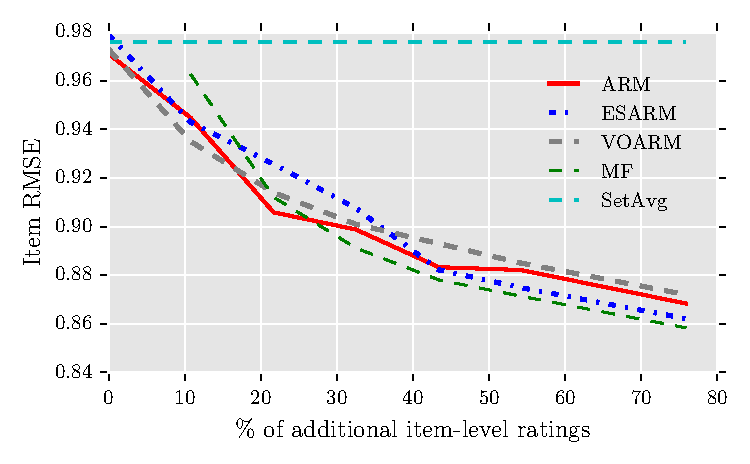
\includegraphics[scale=0.8]{figures/add_items_real_wbias.pdf}}
  \caption{Effect of modeling biases and adding item-level ratings from the same set of users in the real dataset.}
  \label{fig:real_add_items_wbias}
\end{figure}

\begin{figure}[bt]
  \centerline{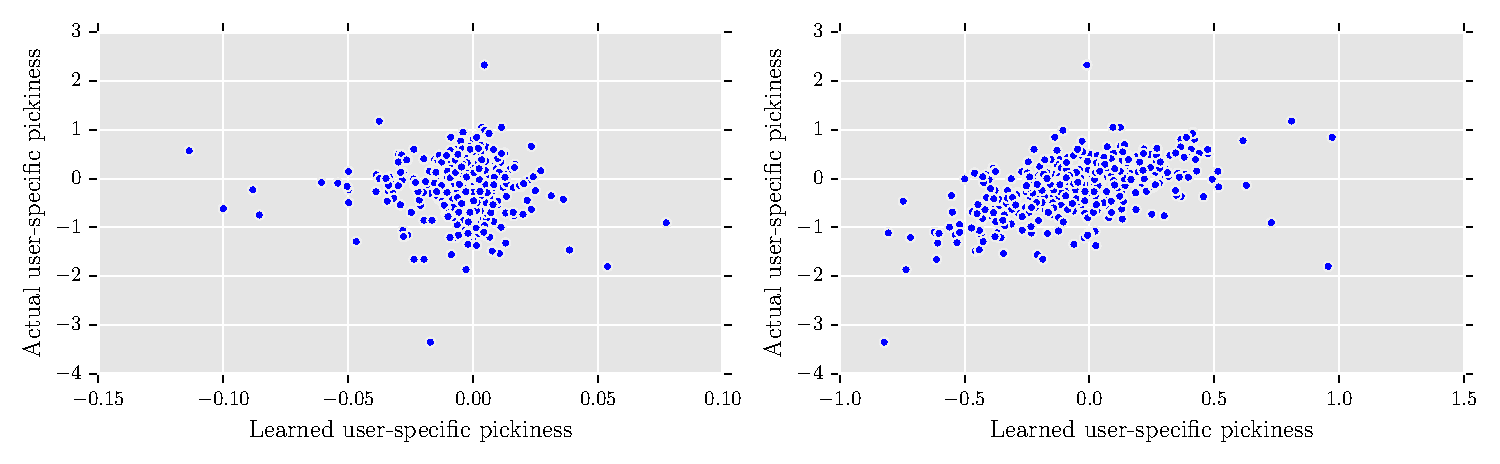
\includegraphics[scale=0.57]{figures/recov_real_mix.pdf}}
  \caption{
    Scatter plots of the user's original level of pickiness computed from real
    data and the pickiness estimated by \VO from set-level ratings (left), and
    after including 30\% of item-level ratings (right).  
  }
  \label{fig:real_add_items_recov}
\end{figure}



\begin{figure}[bt]
  \centerline{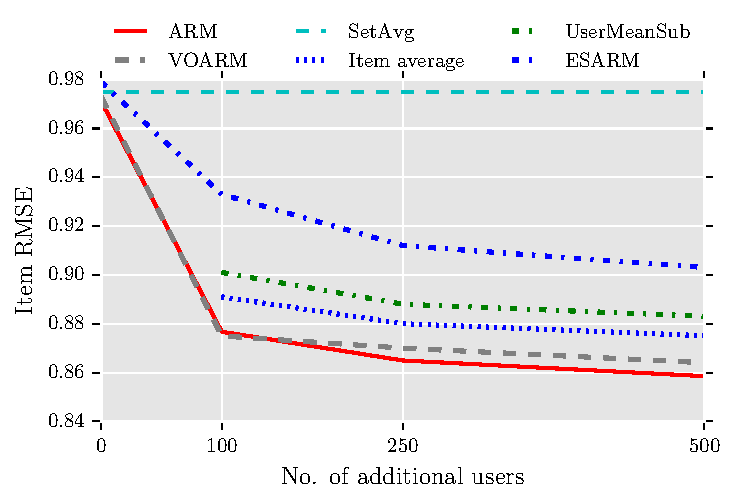
\includegraphics[scale=0.8]{figures/add_users_real_wbias.pdf}}
  \caption{Effect of modeling biases and adding item-level ratings from disjoint set of users in the real dataset.}
  \label{fig:real_add_users_wbias}
\end{figure}


Additionally, we examined the case when we have item-level ratings from the
additional users. 
In addition to estimating ratings from the proposed methods, 
we estimated the ratings at item-level from the two
non-personalized methods, i.e., Item average and UserMeanSub, as described in
Section~\ref{ch:lfs:comp_methods}. 
Figure~\ref{fig:real_add_users_wbias} shows the results for these non-personalized methods along with that of
the proposed methods. As can be seen in the figure, the proposed methods
outperform the non-personalized methods and performance of the proposed
methods continue to improve with the availability of more item-level ratings
from additional users.


\begin{table}[bt]
  \centering
  \caption{RMSE  for item-level predictions for
  additional users, that have provided only the item-level ratings.}
  \label{table:perf_addu_real}
  \begin{threeparttable}
  \def\arraystretch{1.5}

  \begin{tabular}{@{\hspace{10pt}}l@{\hspace{40pt}}c}
    \hline
    Method & Item-level RMSE \\
    \hline
    MF  & 1.003 \\
    \ARM & \underline{0.978} \\
    \ES & 1.043 \\
    \VO & 1.033 \\
    \hline
  \end{tabular}
  \end{threeparttable}
\end{table}


Further, we investigated if using set-level ratings from existing users can
improve the item-level predictions for additional users who have provided
ratings only at item-level. To this end, we selected 500 additional users and
added a random subset of 10 ratings per user from the items that belong to the
sets rated by existing users. 
Table~\ref{table:perf_addu_real} shows the performance of item-level predictions for additional users
after using set-level ratings from the existing users and also shows the
performance of MF method after using only the additional item-level ratings.
As can be seen in the table, \ARM outperforms MF for item-level predictions after
using set-level ratings from existing users. However, \ES and \VO do not
perform better than MF for the additional users. 
Similar to our results on synthetic datasets, it is promising that using
item-level ratings from the additional users and set-level ratings from the
existing users improves the performance not only for latter but also for those
additional users who have provided only item-level ratings. 

%


\subsubsection{Accuracy of item-level predictions for picky
users}\label{ch:lfs:picky_users_analysis}
\begin{table}[bt]
  \centering
  \caption{The item-level RMSE of the proposed methods on different subset of users using
  only set-level ratings and after including additional item-level ratings.}
  \label{table:perf_picky_subsets}
  \begin{threeparttable}
  \def\arraystretch{1.5}
    \begin{tabular}{@{\hspace{8pt}}l@{\hspace{8pt}}c@{\hspace{8pt}}c@{\hspace{8pt}}c@{\hspace{8pt}}c@{\hspace{8pt}}}
      \hline
      & \multicolumn{2}{c}{Set only} & \multicolumn{2}{c}{+Items}\\ 
      
      Method & $U_{Non-picky}$ & $U_{Picky}$ & $U_{Non-picky}$ & $U_{Picky}$ \\
      \hline
      \ARM & \underline{0.915} & 1.089 & \underline{0.879} & 0.975 \\
      \ES & 0.922 & 1.103 & 0.898 & \underline{0.923} \\
      \VO & 0.921 & \underline{1.085} & 0.892 & 0.932 \\
      \hline
    \end{tabular}
  \begin{tablenotes}[para,flushleft]
    The ``Set only'' column denotes the results of the models that were
    estimated using only set-level ratings. The ``+Items'' column show the
    results of the models that were estimated using the sets of ``Set only'' and
    also some additional ratings on a different set of items from the same users
    that provided the set-level ratings.
    $U_{picky}$ refers to the users who have rated at least 20 sets and have a high
    level of pickiness, i.e., $|\beta_u| > 0.5$, in real dataset, and $U_{Non-picky}$ represents
    the remaining users.  
  \end{tablenotes}
  \end{threeparttable}
\end{table}



Even though
\ARM performs better than remaining methods for item-level predictions, we investigated how
well do \ARM, \ES and \VO perform for item-level predictions for the users who have rated at least 20 sets and
have a high level of pickiness, i.e., $|\beta_u| > 0.5$. We found 374 users in the
dataset that were non-picky ($U_{Non-picky}$) and 135 users that were having a higher level of
pickiness ($U_{Picky}$). 
Table~\ref{table:perf_picky_subsets} shows the performance of the proposed
methods for item-level predictions using set-level ratings and after
including 30\% of additional item-level ratings on both $U_{Picky}$ and
$U_{Non-picky}$. As can be seen in the table, for set-level ratings
\VO performs somewhat better than \ARM on $U_{picky}$ and
after including additional item-level ratings  both \ES and \VO
outperform \ARM on $U_{Picky}$.

The overall consistency of the results between the synthetically generated and
the real dataset suggests that \VO and to some extend \ES 
are able to capture the tendency that some users have to consistently under- or
over-rate  diverse sets of items.


